\section{Conclusion}

We now examine the topology of both systems.
Eqs. \eqref{eq:HeffDirac} and \eqref{eq:Heff2deg} are in LL Hamiltonian form, and typically exhibit QHE.
The two systems only have translational symmetry in the $y$-axis, so a Chern number based on periodicity in $k_x$ and $k_y$ is not applicable, though one can relate the center of mass of an electron to the Chern number as shown in Appendix \ref{chern-number}, which is related to the Laughlin pump.
Considering the Laughlin pump argument, both systems have quantized Hall conductivity, since both have the same eigenstates as their respective LL Hamiltonian.
A key difference to note about both systems is the $C$ term in Eq. \eqref{eq:HeffDirac}.
This term will stay positive for the values of $E$ used in the high-frequency limit for the Dirac case.

Using existing experiments \cite{YHW, JWM} we can provide an estimate for the strength of the effective magnetic field to observe LL-like spectrum and QHE.
Analytical structure of Eq.~(\ref{eq:DiracEner}) and Eq.~(\ref{eq:2DEGenergy}) are primarily responsible for the LL-like spectrum in both the Dirac and 2DEG systems, respectively.
Although such results are valid for other 2D materials or Schr\"{o}dinger systems, however, for simplicity, we will consider parameters realized for graphene or topological insulators \cite{YHW, JWM}.
We will consider a similar range of mid-IR photon energies (or $\lambda = [3\mu $m$ , 10\mu $m$]$) as seen in graphene or topological insulators \cite{YHW, JWM} to match with recently proposed high refractive index metamaterial composites \cite{shimFundamentalLimitsRefractive2021}.
In these experiments \cite{YHW, JWM}, the strength of the electric field used is $1 \times 10^7$ V/m to $1 \times 10^8$ V/m, for the parameters used to estimate effective magnetic fields for both systems the largest electric field is around $1.4 \times 10^8$ V/m.
As should be considered, the larger both photon energy and electric field become ultrafast pulses should be used to prevent thermal damage to materials, on the order of $500$ fs.
To note, for the following results we assume a high oblique angle to let $\sin{(\theta_i)} \approx 1$.

To enhance the effective magnetic field, aside from using higher photon energy, reducing the photon phase velocity can see a considerable increase in both systems.
The refractive index materials can be set above graphene, or any Dirac material, such that the lasers can propagate through to reduce its phase velocity.
Germanium refractive index increases monotonically with increasing photon energy, we use a linear interpolation of the refractive index due the small change for the range of photon energies used.
Al-composite metamaterials refractive index is monotonically decreasing with increasing photon energy and we use a linear interpolation here as the data is roughly linear.

\begin{figure}
  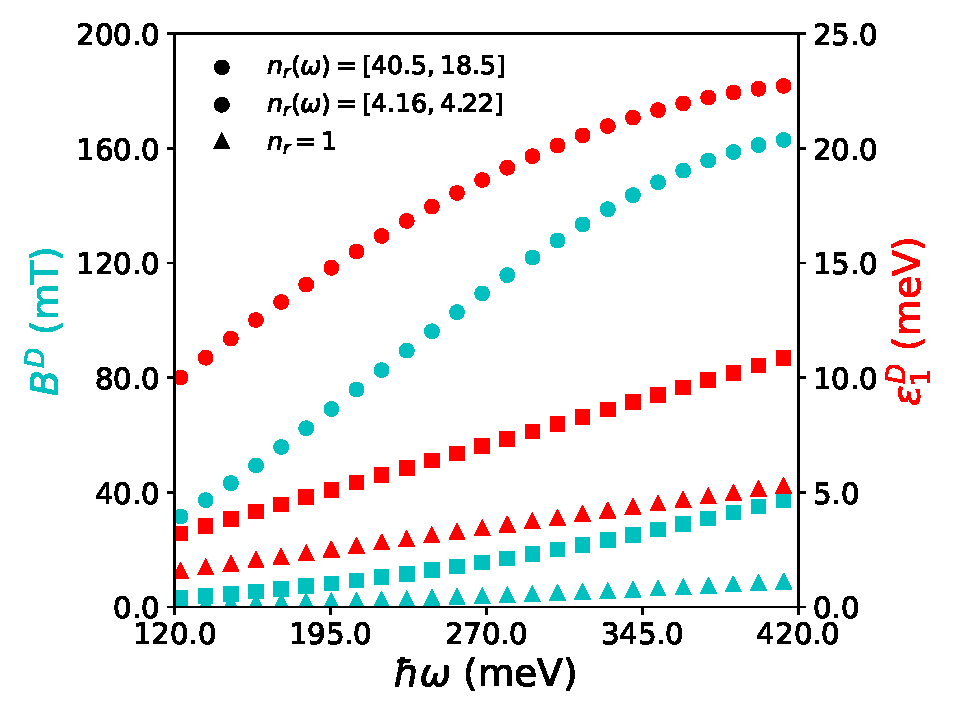
\includegraphics[width=0.45\textwidth]{./figures/dirac-eff-bfield-energy.pdf}
  \caption{Effective magnetic field (cyan) and first quasienergy (red) as a function of photon energy for various refractive materials: vacuum (triangles), germanium (squares), and  Al-composite metamaterial (circles).}
  \label{fig:dirac-bfield-energy}
\end{figure}

In case of a Dirac system Fig. \ref{fig:dirac-bfield-energy} shows graphene with various refractive index materials to enhance the effective magnetic field and first order quasienergy of the LL-like spectrum.
For mid-IR ranges of lasers, the effective magnetic field (cyan) can get up to $8.8$ mT for vacuum, $37.2$ mT for germanium, and $163$ mT for Al-composite metamaterial for $\hbar\omega=413$ meV and results in first order quasienergies (red) of $5.3$ meV, $11$ meV, and $23$ meV, respectively.
As can be seen in \ref{fig:dirac-bfield-energy} as photon energy increases the Al-composite refractive index decreases quite a bit and if we used higher energy we would see the effective magnetic field and quasienergies start to decrease, as will be seen with 2DEG.
While the material has higher index of refraction overall, it would be better to find a material that increases refractive index with photon energy, like germanium can, for it can drastically increase for slightly higher photon energies before effective magnetic field dips \cite{amotchkinaCharacterizationEbeamEvaporated2020}.

\begin{figure}
  \subfloat[]{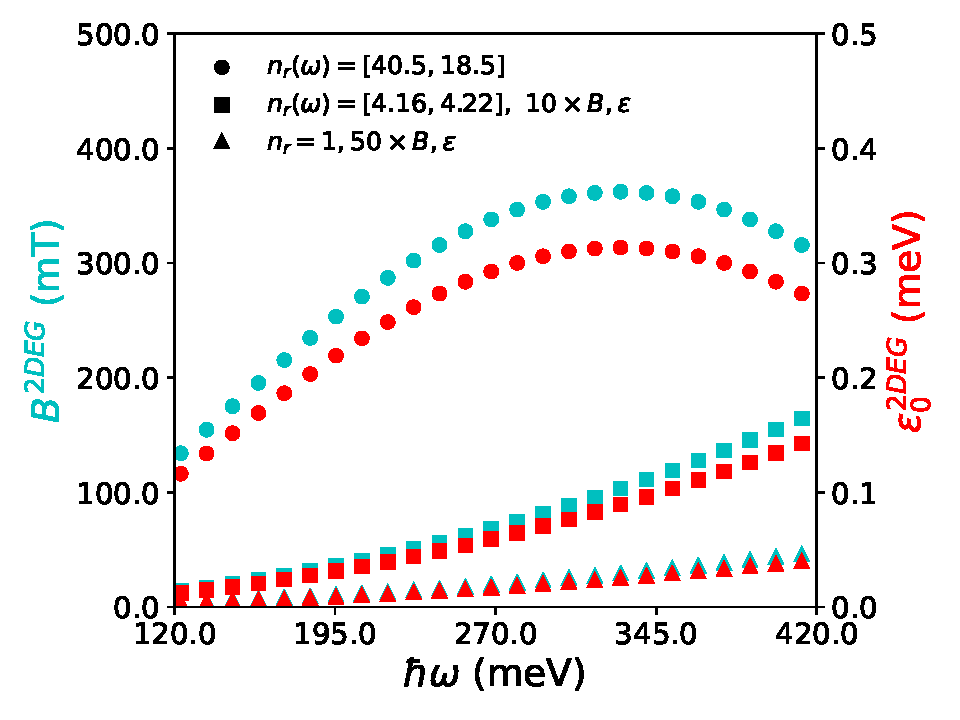
\includegraphics[width=0.45\textwidth]{./figures/2deg-eff-bfield-energy-GaAs.pdf}}
  \subfloat[]{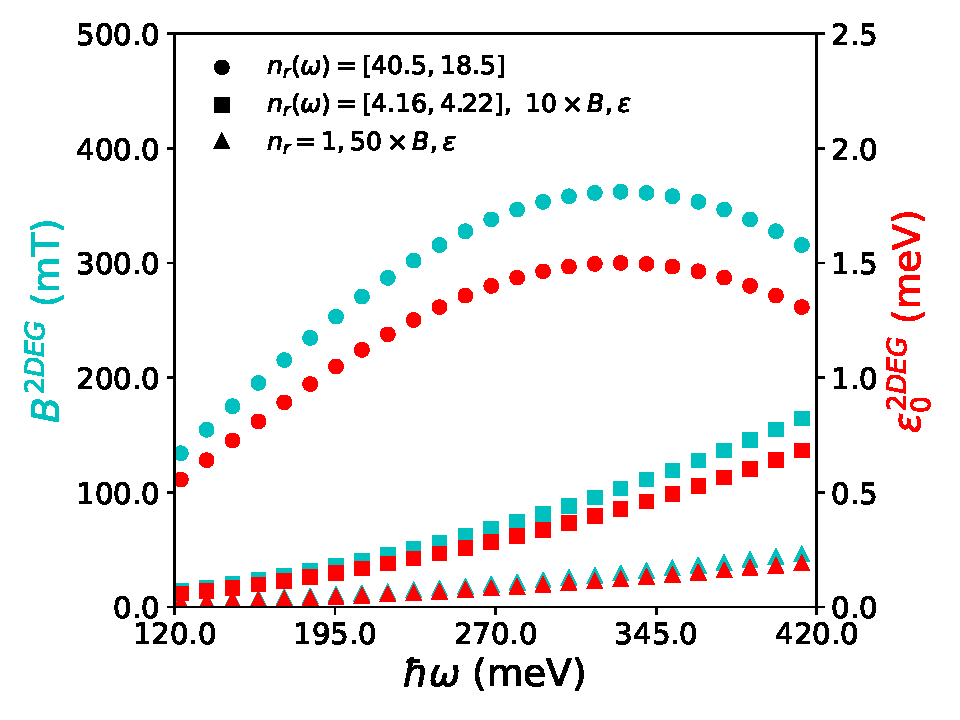
\includegraphics[width=0.45\textwidth]{./figures/2deg-eff-bfield-energy-InSb.pdf}}
  \caption{Effective magnetic field (cyan) and first quasienergy (red) as a function of photon energy for 2DEGs for various refractive materials: vacuum (triangles) scaled by a factor of 50, germanium (squares) scaled by a factor of 10, and Al-composite metamaterials. The 2DEG materials used are (a) GaAs and (b) InSb.}
  \label{fig:2deg-bfield-energy}
\end{figure}

For 2DEG systems Fig. \ref{fig:2deg-bfield-energy} shows GaAs and InSb materials with the same refractive materials used for graphene to enhance effective magnetic field and zeroth order quasienergy of the LL-like spectrum.
The vacuum and germanium interfaces are scaled up by a factor of $10$ and $50$, respectively, to visually enhance and compare it to the Al-composite interface.
GaAs is used as it is one of the most common 2DEG with relatively small effective electron mass, followed by InSb since it has the smallest effective electron mass found in 2DEG materials.
For the GaAs system, effective magnetic field (cyan) can get up to $0.92$ mT for vacuum, $16.5$ mT for germanium, and $362$ mT for Al-composite metamaterial and achieves zeroth order quasienergies (red) of $0.8\ \mu$eV, $14.3\ \mu$eV, and $314\ \mu$eV, respectively.
In the InSb system, effective magnetic field is the same as GaAs, since it has no dependence on effective mass, and achieves zeroth order quasienergies (red) of $3.8\ \mu$eV for vacuum, $68.2\ \mu$eV for germanium, and $1.5$ meV for Al-composite.
As alluded to earlier, due to Al-composites large decrease in refractive index for increasing photon energy, it peaks earlier around $\hbar\omega=328$ mT, for 2DEG.
Overall, we see large changes in 2DEG for both effective magnetic field, due to being proportional to refractive index squared and quasienergies, being inversely proportional to effective electron mass.

There are a few items we did not consider for our calculations.
First, we do not consider any effects due to a refractive index material in contact with a Dirac or 2DEG system.
Secondly, while the high-frequency expansion limits the electric field applied to the materials one could still go beyond the limit of $\hbar \omega \ll H_{pm1}, H_{\pm2}$ to enhance the effective magnetic field by a few orders of magnitude with some error.
For example, if instead we use $\hbar\omega = H_{\pm1}, H_{\pm2}$, this would be multiplying the electric field by a factor of $5$ from our calculations presented, Dirac effective magnetic field would increase by a factor of $125$ while 2DEG effective magnetic field would increase by a factor of $25$.
For Dirac systems with higher electric field strengths, if $C=0$, there would be no QHE as there is no coupling between $x$ and $p_y$, and if $C<0$, the direction of chirality flips.

In conclusion, we have shown Floquet LLs and the QHE using three linearly polarized lasers for Dirac and conventional 2DEG systems.
While using these lasers, we  need at least two polarized lasers to be spatially inhomogeneous and mirrored.
We have presented results using frequency space expansion method and degenerate Floquet perturbation theory.
While, a tight-binding model capable of using ``low-frequency'' with a Peierls substitution can be found in appendix \ref{app:tbm-dirac} and \ref{app:tbm-2deg}, the results are difficult to interpret and currently not informative.
The results agree well to show Floquet LL-like energies in experimentally accessible parameters range.
Also, it is vital to note we are flexible to use different values of the electric field strength, photon energy, or phase velocity to realize QHE and control the strength of the effective magnetic field.
Therefore, we think Floquet LL-like and QHE can be observed in experiments for moderate strength of the spatially inhomogeneous lasers. Moreover, we expect to open up new avenues for nanoelectronics in nonequilibrium systems.


